\documentclass{article}

\usepackage[affil-it]{authblk}
\usepackage{graphicx}
\usepackage{float}
\usepackage[ruled]{algorithm2e}
\usepackage{titlepic}

\graphicspath{{../resources/}}

\SetKwProg{function}{Function}{}{}
\newcommand{\assign}[2]{$#1 \leftarrow$ #2}

\title{COMP390 Evolving a Sorting Algorithm with SNGP}
\author{Robin Lockyer\\{\small Student ID: 201148882 \\ Primary Supervisor: Dr. David Jackson \\ Secondary Supervisor: Dr. Valentina Tamma}}
\date{2018/2019}
\titlepic{\includegraphics[width=0.5\textwidth]{UOL_Logo.png}}

\begin{document}
	
	\maketitle	
	
	\newpage
	
	\begin{abstract}
		
		Genetic programming is a technique for creating programmes not by writing them by hand, but instead by creating a population of random programmes and modifying them using an evolutionary algorithm. The desired result is that after several generations a programme that performs well at a given task is generated. GP has previously been used to successfully evolve sorting algorithms.
		
		Single node genetic programming is a variation on GP invented by Dr Jackson which structures the population of programmes in a manner that allows the use of dynamic programming when computing the result of the programmes in an effort to more efficiently generate a working solution. 
		
		This project aims to compare the effectiveness of the two methods in evolving a sorting algorithm.
		
	\end{abstract}
	\newpage
	\tableofcontents
	\newpage
	\section{Introduction}
	
		This project is was done for my project supervisor Dr David Jackson. The aim of this project is to attempt to evolve a sorting algorithm using node genetic programming (SNGP) and, if successful, compare the effectiveness of evolving sorting algorithms using standard genetic programming (GP) to evolving sorts with SNGP.
		
		The purpose of GP is to automate the creation of algorithms and programmes. This is done by applying a genetic algorithm to a population of random programmes so that successive generations of programmes improve at the desired characteristics until a functional programme is created.
		The standard approach to GP requires evaluating hundreds of programmes per generation over potentially thousands of generations and as such GP can take up a large amount of processing time. Several variations of GP have been created that try to reduce the amount of processing, including Linear Genetic Programming and Parallel Distributed GP \cite{poli_field_2008}.
		
		SNGP is one such variation devised by Dr Jackson in \textit{A New, Node-Focused Model for Genetic Programming} \cite{jackson_new_2012}. This variation makes use of a form of dynamic programming to re-use results of previously evaluated programmes. It has been shown that SNGP tends to perform better than standard GP in terms of processing time, solution rate, and solution size \cite{jackson_new_2012}. SNGP has reduced efficiency when dealing with problems with side-effects because this prevents re-use of evaluations, although it still performs better than GP at some problems with side effects \cite{jackson_single_2012}. 
		
		A sorting algorithm reads and manipulates an array of integers as it executes, and so must make use of side effects. Regular genetic programming has been shown to be capable of evolving a working sorting algorithm \cite{kinnear_evolving_1993,kinnear_generality_1993}. This makes evolving a sort a good problem to evaluate SNGP on as comparisons can be made with previous research.
	
	\section{Background}
	
		\subsection{Standard Genetic Programming}
		
			In standard GP, programmes are encoded as a tree of primitive functions and terminals.
			
			\begin{figure}[H]
				\centering
				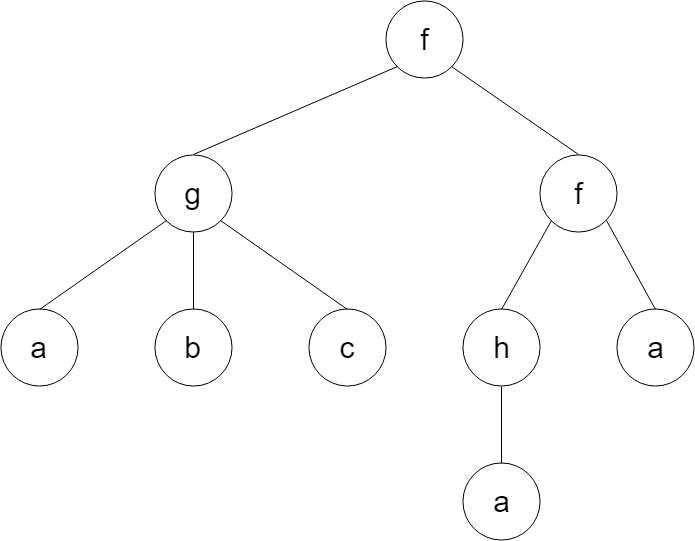
\includegraphics[width=0.5\textwidth]{1_gp_example_tree}
				\label{fig:ex_prog_tree}
				\caption{This tree encodes the programme f( g( a, b, c ), f( h( a ), a ) ), where f, g, and h are functions and a, b, and c are terminals.}
			\end{figure}
			
			An initial population of random programmes is created
			
			\begin{figure}[H]
				\centering
				
\includegraphics[width=0.5\textwidth]{2_gp_example_population}
				\caption{An example GP population}
			\end{figure}
		
			Each member of the population is executed, evaluated, and given a fitness score
			
			\begin{figure}[H]
				\centering
				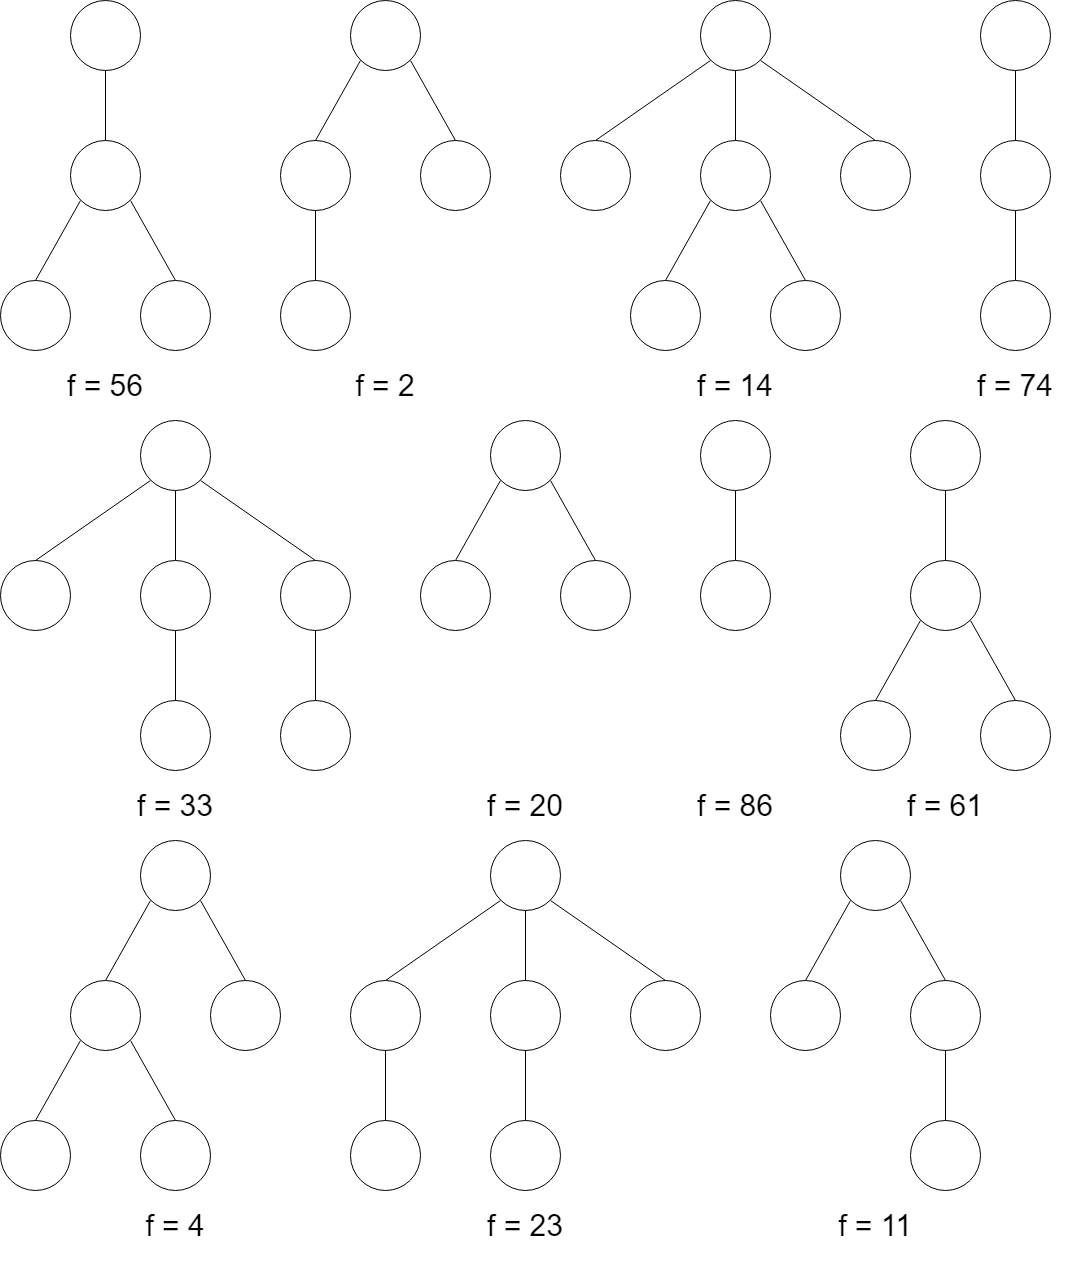
\includegraphics[width=0.5\textwidth]{3_gp_example_fitness}
				\caption{An example GP population with fitness scores}
			\end{figure}
		
			A new population is created by selecting some of the most fit members of the initial population and performing genetic operations on them to create new programmes.
			
			\begin{figure}[H]
				\centering
				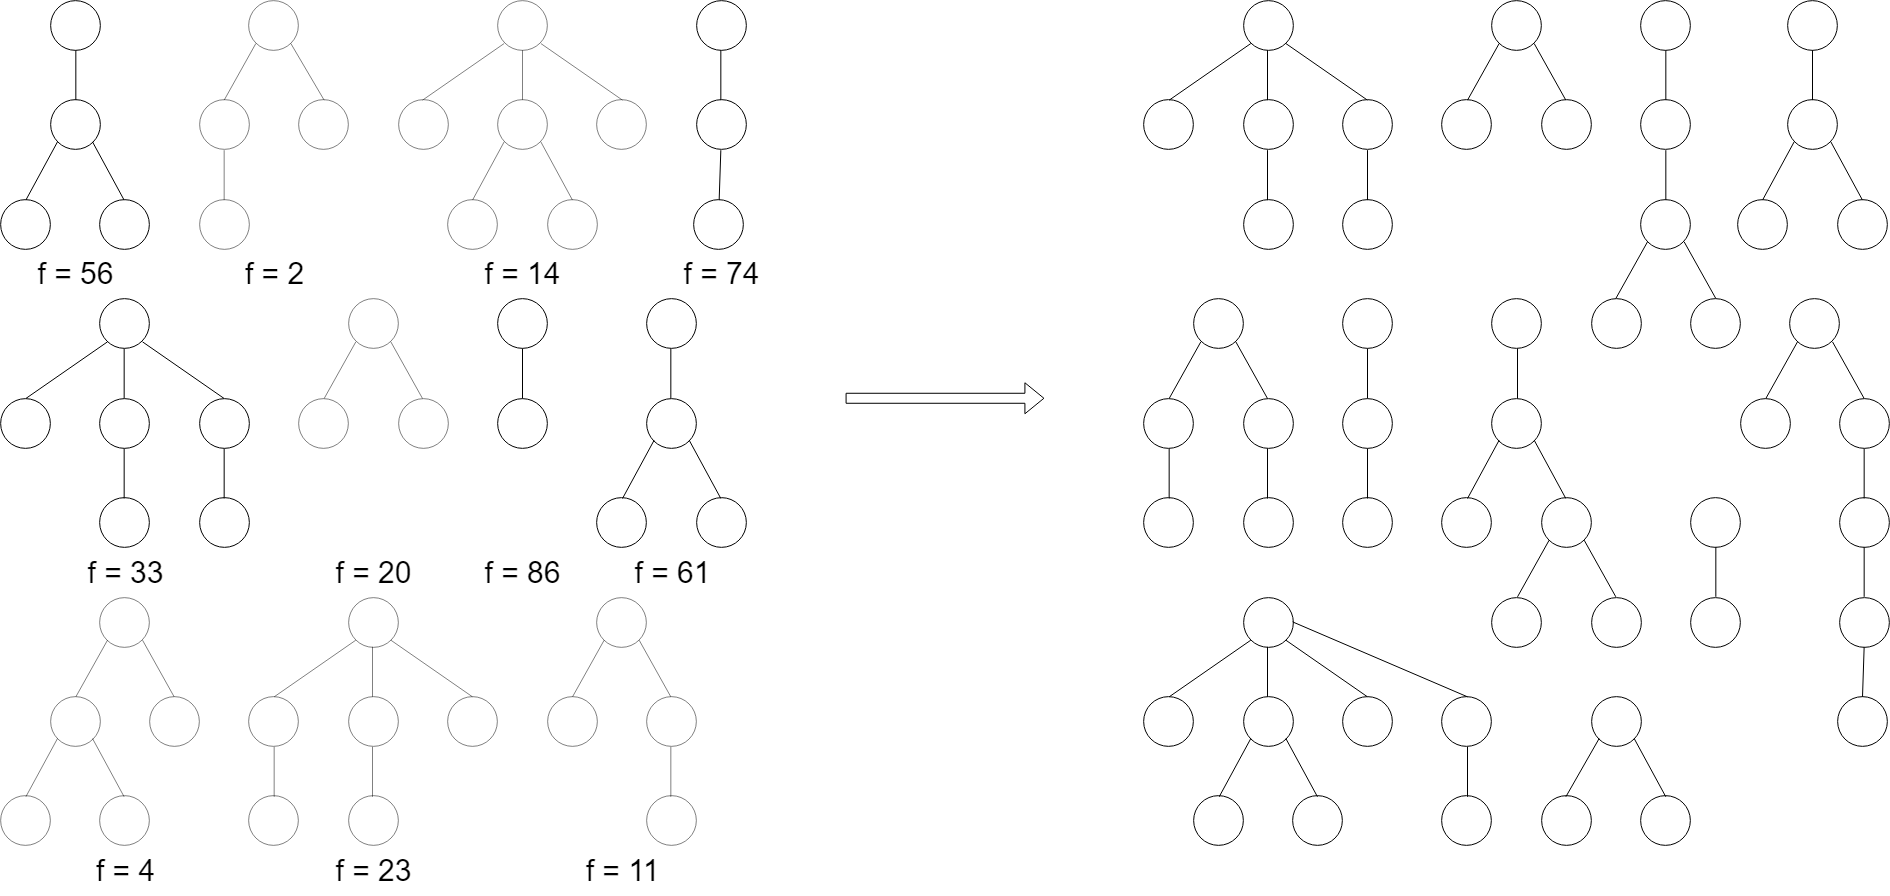
\includegraphics[width=0.5\textwidth]{4_gp_example_selection}
				\caption{An example GP population with fitness scores}
			\end{figure}
			
		\subsection{Single Node Genetic Programming}
		 
		
	
	\section{Data Required}
	
	\section{Design}
	
		\subsection{GP Implementation}
		
		The GP implementation was based example code given by Dr Jackson and also on an implementation of the TinyGP system found in the book \textit{A Field Guide to Genetic
		Programming} \cite{poli_field_2008}. It was written in C as the example code given to me was also in C. The exact parameters are the same as described in Koza's work \cite{kinnear_generality_1993}.
		
		Each programme is stored as a string of primitive functions and terminals. The string is in prefix notation, and as all primitives have fixed arity no bracketing is needed. Executing a programme is done by a recursive interpreter 
		
		The each member of the population is initialised by using the grow method. A maximum tree depth is specified and a random primitive is selected as the root. Random primitives are selected as the children for primitives that have been previously selected. The primitives can be either functions or terminals, unless selecting a function would cause the tree to exceed the maximum depth. The initial maximum depth is chosen to be 6 to match Koza's work. The pseudocode for the algorithm is shown in
		
		\begin{algorithm}
			\KwIn{maxTreeDepth}
		\end{algorithm}
	
		Three genetic operators are used: crossover, reproduction, and mutation. 
		
		\begin{algorithm}[H]
			
			$initialisePopulation()$
			
			$evaluatePopulation(0)$
			
			\For{$generation \leftarrow 1$ \KwTo $NUM\_GENERATIONS$}{
				
				\For{$j \leftarrow$  \KwTo $POPULATION\_SIZE$}{
					
					\uIf{$randInt(1,10) <= 8$}{
					
						$newPopulation[j] \leftarrow crossover(selectProg(),selectProg())$
						
					}
					\Else{$newPopulation[j] \leftarrow reproduce(selectProg())$ }
					
				}
			
				\ForEach{$programme \in newPopulation$}{
					
					\If{$randInt(1,10) = 1$}{
						
						$mutate(programme)$
						
					}
			
				}
			
				$population \leftarrow newPopulation$
			
				$evaluatePopulation(generation)$
		
			}
		
			\KwOut{$best(population)$}
				
			\caption{Genetic Programming Algorithm}
			
			\label{alg:GP}
		\end{algorithm}
		
		\subsection{SNGP Implementation}
		
		\subsection{Fitness Functions}
		
			While many different fitness functions were used, they all counted the number of inversions in a test array before and after executing a programme. To efficiently count inversions I used a modified merge sort algorithms, detailed in algorithm \ref{alg:countInv}. The algorithm is $O(n\log{}n)$, and merging is done using two preallocated buffers to avoid unnecessary memory allocations while the GP algorithm is running.
			
			\begin{algorithm}
				
				\SetKw{countInversions}{countInversions}
				
				\function{\countInversions{$(arr)$}:}{
				
					\uIf{$length(arr) <= 1$}{
						
						\assign{inversions}{$0$}
				
					}
				
					\Else{
					
						\assign{sizeA}{$\left\lfloor length(arr) / 2 \right\rfloor$}
						
						\assign{sizeB}{length(arr) - sizeA}
						
						\assign{A}{[First sizeA elements of arr]}
						
						\assign{B}{[Last sizeB elements of arr]}
						
						\assign{inversions}{countInversions(A) + countInversions(B)}
						
						\assign{C}{Empty Array}
						
						\While{$length(A) > 0 and length(B) > 0$}{
						
							\uIf{$B[1] < A[1]$}{
								
								Append B[1] to C
								
								\assign{inversions}{inversions + length(A)}
								
								Remove first element of B
						
							}
							\Else{
							
								Append A[1] to C
								
								Remove first element of A
							
							}
						}
						
						\uIf{$length(A) = 0$}{
						
							Append remaining elements of B to C
						
						}
						\ElseIf{$length(B) = 0$}{
							Append remaining elements of A to C
						}
					
						\assign{arr}{C}
				
					}
				
					\KwOut{inversions}
			
				}
				
				\caption{Algorithm that sorts array and counts number of inversions}
				
				\
				
				\label{alg:countInv}
				
			\end{algorithm}
		
		\subsection{Test Data}
		
			Each programme generated during a GP run is executed on a set of test arrays. This data comes from pre-generated file containing a series of random arrays loaded into the programme at the beginning of execution. This has the advantage of allowing for reproduction of results, easier testing of the programme, and prevents random number generation from increasing the execution time.
			
			The arrays are organised into fixed size groupings. Each programme in the same GP generation is executed on the same group of arrays. This was done so that each programme was subjected to the same conditions in each generation, while still preventing over fitting to a fixed set of data. This method also allows each group to be customized to meet certain requirements (e.g. contains a sorted array, a reversed array, or a very short array), but this was found to be unnecessary.
			
			The file is a standard text file where the first two values on each line are the length and number of inversions of the array, followed by the array itself. Each value is separated by a space. A blank line indicates the end of the current group of arrays.
	
	\section{Realisation}
	
	\section{Results}
	
	
	
	\section{Evaluation}
	
	\section{Learning Points}
	
	\section{Professional Issues}
	
	\section{Bibliography}
	
		\bibliographystyle{acm}
		\bibliography{library}
	
	\section{Appendices}
		
\end{document}